\section{Generalizable Robustness by Confidence Calibration of Adversarial Training}
\label{sec:main}

To start, we briefly review adversarial training on $L_\infty$ adversarial examples \cite{MadryICLR2018}, which has become standard to train robust models, \cf \secref{sec:main-at}.
However, robustness does not generalize to larger perturbations or unseen attacks. We hypothesize this to be the result of enforcing high-confidence predictions on adversarial examples.
\ConfTrain addresses this issue with minimal modifications, \cf \secref{subsec:main-ccat} and \algref{alg:main-ccat}, by encouraging low-confidence predictions on adversarial examples. During testing, adversarial examples can be rejected by confidence thresholding.

\textbf{Notation:}
%
We consider a classifier $f:\R^d \rightarrow \R^K$ with $K$ classes where $f_k$ denotes the confidence for class $k$. While we use the cross-entropy loss $\cL$ for training, our approach also generalizes to other losses. Given $x \in \R^d$ with class $y{\,\in\,}\{1,\ldots,K\}$, we let $f(x) :=\argmax_k f_k(x)$ denote the predicted class for notational convenience. For $f(x) = y$, an adversarial example $\tilde{x} = x+\delta$ is defined as a ``small'' perturbation $\delta$ such that $f(\tilde{x}) \neq y$, \ie, the classifier changes its decision. The strength of the change $\delta$ is measured by some $L_p$-norm, $p \in \{0,1,2,\infty\}$. Here, $p=\infty$ is a popular choice as it leads to the smallest perturbation per pixel.

\subsection{Problems of Adversarial Training}
\label{sec:main-at}

Following \cite{MadryICLR2018}, adversarial training is given as the following min-max problem:
\vspace*{0px}
\begin{align}
    \min\limits_w \Exp\left[\max\limits_{\|\delta\|_\infty \leq \epsilon}\, \cL(f(x + \delta; w), y)\right]\label{eq:adversarial-training}
\end{align}
\vskip -4px
with $w$ being the classifier's parameters. During mini-batch training the inner maximization problem,
\vspace*{0px}
\begin{align}
    \max\limits_{\|\delta\|_\infty \leq \epsilon} \cL(f(x + \delta; w), y),\label{eq:attack}
\end{align}
\vskip -4px
is approximately solved. In addition to the $L_\infty$-constraint, a box constraint is enforced for images, \ie, $\tilde{x}_i = (x + \delta)_i \in [0,1]$. Note that maximizing the cross-entropy loss is equivalent to finding the adversarial example with \emph{minimal} confidence in the true class. For neural networks, this is generally a non-convex optimization problem. In \citep{MadryICLR2018} the problem is tackled using projected gradient descent (\PGD), initialized using a random $\delta$ with $\|\delta\|_\infty \leq \epsilon$.

In contrast to adversarial training as proposed in \citep{MadryICLR2018}, which computes adversarial examples for the \emph{full} batch in each iteration, others compute adversarial examples only for \emph{half} the examples of each batch \citep{SzegedyICLR2014}. Instead of training \emph{only} on adversarial examples, each batch is divided into $50\%$ clean and $50\%$ adversarial examples. Compared to \eqnref{eq:adversarial-training}, $50\%$/$50\%$ adversarial training effectively minimizes
\vspace*{0px}
\begin{align}
    \underbrace{\Exp\Big[\max\limits_{\|\delta\|_\infty \leq \epsilon} \cL(f(x + \delta; w), y)\Big]}_{\text{50\% adversarial training}} + \underbrace{\Exp\big[\cL(f(x; w), y)\big]}_{\text{50\% ``clean'' training}}.\label{eq:50-50-adversarial-training}
\end{align}
\vskip -4px
This improves test accuracy on clean examples compared to $100\%$ adversarial training but typically leads to worse robustness. Intuitively, by balancing both terms in \eqnref{eq:50-50-adversarial-training}, the trade-off between accuracy and robustness can already be optimized to some extent \citep{StutzCVPR2019}.

\begin{figure}[t]
    \vspace*{-8px}
    
    \centering
    \begin{minipage}{0.49\textwidth}
        \hspace*{-0.2cm}
        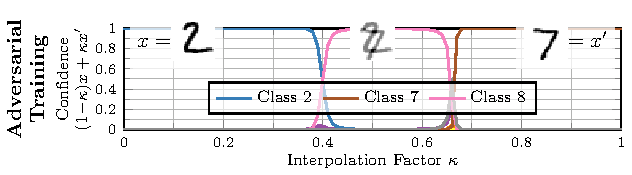
\includegraphics[width=1\textwidth]{fig_mmnist_advtrain_0_interpolation}
        
        \hspace*{-0.2cm}
        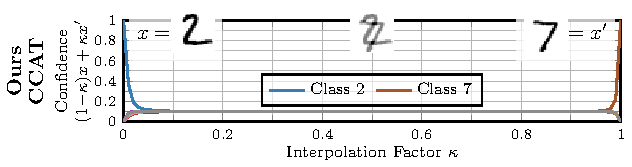
\includegraphics[width=1\textwidth]{fig_mmnist_ours10_0_interpolation}
    \end{minipage}
    \vspace*{-10px}
    
    \caption{\textbf{Extrapolation of Uniform Predictions.} We plot the confidence in each class along an interpolation between two test examples $x$ and $x'$, ``2'' and ``7'', on MNIST \cite{LecunIEEE1998}: $(1 - \kappa)x + \kappa x'$ where $\kappa$ is the interpolation factor. \ConfTrain quickly yields low-confidence, uniform predictions in between both examples, extrapolating the behavior enforced within the $\epsilon$-ball during training. Regular adversarial training, in contrast, consistently produces high-confidence predictions, even on unreasonable inputs.}
    \label{fig:interpolation}
    \vspace*{-2px}
\end{figure}

\textbf{Problems:}
%
Trained on $L_\infty$ adversarial examples, the robustness of adversarial training does not generalize to previously unseen adversarial examples, including larger perturbations or other $L_p$ adversarial examples. We hypothesize that this is because adversarial training explicitly enforces high-confidence predictions on $L_\infty$ adversarial examples within the $\epsilon$-ball seen during training (``seen'' in \figref{fig:introduction}). However, this behavior is difficult to extrapolate to arbitrary regions in a meaningful way. Thus, it is not surprising that adversarial examples can often be found right beyond the $\epsilon$-ball used during training, \cf \figref{fig:introduction} (top left). This can be described as ``overfitting'' to the $L_\infty$ adversarial examples used during training. Also, larger $\epsilon$-balls around training examples might include (clean) examples from other classes. Then, \eqnref{eq:attack} will focus on these regions and reduce accuracy as considered in our theoretical toy example, see Proposition \ref{prop:toy-example}, and related work \citep{JacobsenICLR2019,JacobsenARXIV2019}.

As suggested in \figref{fig:introduction}, both problems can be addressed by enforcing low-confidence predictions on adversarial examples in the $\epsilon$-ball. In practice, we found that the low-confidence predictions on adversarial examples within the $\epsilon$-ball are extrapolated beyond the $\epsilon$-ball, \ie, to larger perturbations, unseen attacks or distal adversarial examples. This allows to reject adversarial examples based on their low confidence. We further enforce this behavior by explicitly encouraging a ``steep'' transition from high-confidence predictions (on clean examples) to low-confidence predictions (on adversarial examples). As result, the (low-confidence) prediction is almost flat close to the boundary of the $\epsilon$-ball. Additionally, there is no incentive to deviate from the uniform distribution outside of the $\epsilon$-ball. For example, as illustrated in \figref{fig:interpolation}, the confidence stays low in between examples from different classes and only increases if necessary, \ie, close to the examples.

\begin{algorithm}[t]
	\caption{\textbf{Confidence-Calibrated Adversarial Training (\ConfTrain).}  The only changes compared to standard adversarial training are the attack (line \ref{line:attack}) and the probability distribution over the classes (lines \ref{line:lambda} and \ref{line:label}), which becomes more uniform as distance $\norm{\delta}_\infty$ increases. During testing, low-confidence (adversarial) examples are rejected.}
	\label{alg:main-ccat}
	\begin{algorithmic}[1]
		\WHILE{true}
		\STATE choose random batch $(x_1,y_1),\ldots,(x_B,y_B)$.
		\FOR{$b = 1,\ldots,\nicefrac{B}{2}$} 
		\STATE $\delta_b:=\argmax\limits_{\|\delta\|_\infty \leq \epsilon} \max\limits_{k \neq y_b} f_k(x_b{+}\delta)$\label{line:attack} (\eqnref{eq:conf-attack})
		\STATE $\tilde{x}_b := x_b + \delta_b$
		\STATE $\lambda(\delta_b) := (1 - \min(1, \nicefrac{\|\delta_b\|_\infty}{\epsilon}))^\rho$ (\eqnref{eq:lambda})\label{line:lambda}
		\STATE $\tilde{y_b}\,{:=}\,\lambda(\delta_b)\,\text{one\_hot}(y_b)\,{+}\,(1\,{-}\,\lambda(\delta_b)) \frac{1}{K}$ (\eqnref{eq:distribution})\label{line:label}
		\ENDFOR
		\STATE update parameters using \eqnref{eq:50-50-adversarial-training}:\\\hspace*{1cm}$\sum_{b = 1}^{\nicefrac{B}{2}} \mathcal{L}(f(\tilde{x}_b), \tilde{y}_b) + \sum_{b = \nicefrac{B}{2}}^{B} \mathcal{L}(f(x_b), y_b)$
		\ENDWHILE
	\end{algorithmic}
\end{algorithm}

\subsection{Confidence-Calibrated Adversarial Training}
\label{subsec:main-ccat}

\textbf{Confidence-calibrated adversarial training (\ConfTrain)} addresses these problems with minimal modifications, as outlined in \algref{alg:main-ccat}. During training, we train the network to predict a convex combination of (correct) one-hot distribution on clean examples and uniform distribution on adversarial examples as target distribution within the cross-entropy loss. During testing, adversarial examples can be rejected by confidence thresholding: adversarial examples receive near-uniform confidence while test examples receive high-confidence. By extrapolating the uniform distribution beyond the $\epsilon$-ball used during training, previously unseen adversarial examples such as larger $L_\infty$ perturbations can be rejected, as well. In the following, we first introduce an alternative objective for generating adversarial examples. Then, we specifically define the target distribution, which becomes more uniform with larger perturbations $\|\delta\|_\infty$. In \algref{alg:main-ccat}, these changes correspond to lines \ref{line:attack}, \ref{line:lambda} and \ref{line:label}, requiring only few lines of code in practice.

Given an example $x$ with label $y$, our adaptive attack during training maximizes the confidence in any other label $k \neq y$. This results in effective attacks against \ConfTrain, as \ConfTrain will reject low-confidence adversarial examples:
\vspace*{0px}
\begin{align}
 \max\limits_{\|\delta\|_\infty \leq \epsilon} \max\limits_{k\neq y}f_k(x + \delta;w) \label{eq:conf-attack}
\end{align}
\vskip -4px
Note that \eqnref{eq:attack}, in contrast, minimizes the confidence in the true label $y$. Similarly, \citep{GoodfellowOPENREVIEW2019} uses targeted attacks in order to maximize confidence, whereas ours is untargeted and, thus, our objective is the maximal confidence over all other classes.

Then, given an adversarial example from \eqnref{eq:conf-attack} during training, \ConfTrain uses the following combination of uniform and one-hot distribution as target for the cross-entropy loss:
\vspace*{-8px}
\begin{align}
	\tilde{y} = \lambda(\delta) \,\,\text{one\_hot}(y) + \big(1-\lambda(\delta)\big) \frac{1}{K},\label{eq:distribution}
\end{align}
\vskip -4px
with $\lambda(\delta) \in [0,1]$ and $\text{one\_hot}(y) \in \{0,1\}^K$ denoting the one-hot vector corresponding to class $y$. Thus, we enforce a convex combination of the original label distribution and the uniform distribution which is controlled by the parameter~$\lambda = \lambda(\delta)$, computed given the perturbation~$\delta$. We choose $\lambda$ to decrease with the distance $\|\delta\|_\infty$ of the adversarial example to the attacked example $x$ with the intention to enforce uniform predictions when $\|\delta\|_\infty = \epsilon$. Then, the network is encouraged to extrapolate this uniform distribution beyond the used $\epsilon$-ball. Even if extrapolation does not work perfectly, the uniform distribution is much more meaningful for extrapolation to arbitrary regions as well as regions between classes compared to high-confidence predictions as encouraged in standard adversarial training, as demonstrated in \figref{fig:interpolation}. For controlling the trade-off $\lambda$ between one-hot and uniform distribution, we consider the following ``power transition'':
\vspace*{0px}
\begin{align}
    \begin{split}
        \lambda(\delta) :=& \Big(1 - \min\Big(1, \frac{\|\delta\|_\infty}{\epsilon}\Big)\Big)^\rho
    \end{split}\label{eq:lambda}
\end{align}
\vskip -4px
This ensures that for $\delta = 0$ we impose the original (one-hot) label. For growing $\delta$, however, the influence of the original label decays proportional to $\|\delta\|_\infty$. The speed of decay is controlled by the parameter $\rho$.
For $\rho=10$, \figref{fig:introduction} (top right) shows the transition as approximated by the network.
The power transition ensures that for $\|\delta\|_\infty \geq \epsilon$, \ie, perturbations larger than encountered during training, a uniform distribution is enforced as $\lambda$ is $0$. We train on $50\%$ clean and $50\%$ adversarial examples in each batch, as in \eqnref{eq:50-50-adversarial-training}, such that the network has an incentive to predict correct labels.

The convex combination of uniform and one-hot distribution in \eqnref{eq:distribution} resembles the label smoothing regularizer introduced in \cite{SzegedyCVPR2016}. In concurrent work, label smoothing has also been used as regularizer for adversarial training \cite{ChengARXIV2020}. However, in our case, $\lambda = \lambda(\delta)$ from \eqnref{eq:lambda} is not a fixed hyper-parameter as in \cite{SzegedyCVPR2016,ChengARXIV2020}. Instead, $\lambda$ depends on the perturbation $\delta$ and reaches zero for $\|\delta\|_\infty = \epsilon$ to encourage low-confidence predictions beyond the $\epsilon$-ball used during training. Thereby, $\lambda$ explicitly models the transition from one-hot to uniform distribution.

\subsection{Confidence-Calibrated Adversarial Training Results in Accurate Models}
\label{sec:main-proposition}

Proposition \ref{prop:toy-example} discusses a problem where standard adversarial training is unable to reconcile robustness and accuracy while \ConfTrain is able to obtain \emph{both} robustness and accuracy:

\begin{proposition}\label{prop:toy-example}
    We consider a classification problem with two points $x=0$ and $x=\epsilon$ in $\mR$ with deterministic labels, \ie,
    $p(y=2|x=0)=1$ and $p(y=1|x=\epsilon)=1$, such that the problem is fully determined by the probability $p_0=p(x=0)$. 
    The Bayes error of this classification problem is zero. Let the predicted probability distribution over classes be $\tilde{p}(y|x)=\frac{e^{g_y(x)}}{e^{g_1(x)}+e^{g_2(x)}}$, where $g:\R^d \rightarrow \R^2$ is the classifier and we assume that the function $\lambda:\mR_+ \rightarrow [0,1]$ used in \ConfTrain is monotonically decreasing and $\lambda(0)=1$. Then, the error of the Bayes optimal classifier (with cross-entropy loss) for
    \vspace*{-8px}
    \begin{itemize}
    \item adversarial training on $100\%$ adversarial examples, \cf \eqnref{eq:adversarial-training}, 
    is $\min\{p_0,1-p_0\}$.
    \vspace*{-3px}
    \item adversarial training on $50\%$/$50\%$ adversarial/clean examples per batch, \cf \eqnref{eq:50-50-adversarial-training}, 
    is $\min\{p_0,1 - p_0\}$.
    \vspace*{-3px}
    \item \ConfTrain on $50\%$ clean and $50\%$ adversarial examples, \cf \algref{alg:main-ccat}, 
    is \emph{zero} 
    if $\lambda(\epsilon) < \min\left\{\nicefrac{p_0}{1-p_0},\nicefrac{1-p_0}{p_0}\right\}$.
    \vspace*{-6px}
    \end{itemize}
\end{proposition}

Here, $100\%$ and $50\%$/$50\%$ standard adversarial training are unable to obtain \emph{both} robustness and accuracy: The $\epsilon$-ball used during training contains examples of different classes such that adversarial training enforces high-confidence predictions in contradicting classes. \ConfTrain addresses this problem by encouraging low-confidence predictions on adversarial examples within the $\epsilon$-ball. Thus, \ConfTrain is able to improve accuracy while preserving robustness.

\section{Detection and Robustness Evaluation with Adaptive Attack}
\label{sec:evaluation-attack}

\ConfTrain allows to reject (adversarial) inputs by confidence-thresholding before classifying them. As we will see, this ``reject option'', is also beneficial for standard adversarial training (\AdvTrain). Thus, evaluation also requires two stages: First, we fix the confidence threshold at $99\%$ true positive rate (TPR), where correctly classified clean examples are positives such that at most $1\%$ (correctly classified) clean examples are rejected.
Second, on the non-rejected examples, we evaluate accuracy and robustness using \emph{confidence-thresholded} (robust) test error. 

\subsection{Adaptive Attack}
\label{subsec:evaluation-attack}

As \ConfTrain encourages low confidence on adversarial examples, we use \PGD to maximize the confidence of adversarial examples, \cf \eqnref{eq:conf-attack}, as effective adaptive attack against \ConfTrain. In order to effectively optimize our objective, we introduce a simple but crucial improvement: after each iteration, the computed update is only applied if the objective is improved; otherwise the learning rate is reduced.
Additionally, we use momentum \citep{DongCVPR2018} and run the attack for exactly $T$ iterations, choosing the perturbation corresponding to the best objective across all iterations. In addition to random initialization, we found that $\delta = 0$ is an effective initialization against \ConfTrain. We applied the same principles for \cite{IlyasICML2018}, \ie, \PGD with approximated gradients, \eqnref{eq:conf-attack} as objective, momentum and backtracking; we also use \eqnref{eq:conf-attack} as objective for the black-box attacks of \cite{AndriushchenkoARXIV2019,NarodytskaCVPRWORK2017,KhouryARXIV2018}.

\subsection{Detection Evaluation}

In the first stage, we consider a detection setting: adversarial example are \emph{negatives} and correctly classified clean examples are \emph{positives}. The confidence threshold $\tau$ is chosen extremely conservatively by requiring a \textbf{$\boldsymbol{99\%}$ true positive rate (TPR)}: at most $1\%$ of correctly classified clean examples can be rejected. As result, the confidence threshold is determined \emph{only} by correctly classified clean examples, independent of adversarial examples. Incorrectly rejecting a significant fraction of correctly classified clean examples is unacceptable. This is also the reason why we do not report the area under the receiver operating characteristic (ROC) curve as related work \citep{LeeNIPS2018,MaICLR2018}.
Instead, we consider the \textbf{false positive rate (FPR)}.
The supplementary material includes a detailed discussion.

\subsection{Robustness Evaluation}

In the second stage, after confidence-thresholding, we consider the widely used robust test error (\RTE) \cite{MadryICLR2018}. It quantifies the model's test error in the case where all test examples are allowed to be attacked, \ie, modified within the chosen threat model, \eg, for $L_p$:
\begin{align}
    \text{``Standard'' }\RTE = \frac{1}{N}\sum_{n = 1}^N \;\max\limits_{\|\delta\|_p\leq \epsilon} \Id_{f(x_n + \delta)\neq y_n}
\end{align}
where $\{(x_n,y_n)\}_{n = 1}^N$ are test examples and labels. In practice, \RTE is computed empirically using adversarial attacks. Unfortunately, standard \RTE does not take into account the option of rejecting (adversarial) examples.

We propose a generalized definition adapted to our confidence-thresholded setting where the model can reject examples. For fixed confidence threshold $\tau$ at $99\%$TPR, the \textbf{confidence-thresholded \RTE} is defined as
\begin{align}
    \RTE(\tau) = \frac{
    	\sum\limits_{n=1}^N \;\max\limits_{\|\delta\|_p\leq \epsilon, c(x_n + \delta)\geq \tau} \Id_{f(x_n + \delta)\neq y_n}
    }
    {
    	\sum\limits_{n=1}^N \;\max\limits_{\|\delta\|_p\leq \epsilon} \Id_{c(x_n + \delta)\geq \tau}
    }\label{eq:conf-rte}
\end{align}
with $c(x) = \max_k f_k(x)$ and $f(x)$ being the model's confidence and predicted class on example $x$, respectively. Essentially, this is the \textbf{test error on test examples that can be modified within the chosen threat model \emph{and} pass confidence thresholding}. For $\tau=0$ (\ie, all examples pass confidence thresholding) this reduces to the standard \RTE, comparable to related work. We stress that our adaptive attack in \eqnref{eq:conf-attack} directly maximizes the numerator of \eqnref{eq:conf-rte} by maximizing the confidence of classes not equal $y$. A (clean) \textbf{confidence-thresholded test error ($\TE(\tau)$)} is obtained similarly. In the following, if not stated otherwise, we report \emph{confidence-thresholded} \RTE and \TE as default and omit the confidence threshold $\tau$ for brevity.

\textbf{FPR and \RTE:}
%
FPR quantifies how well an adversary can perturb (correctly classified) examples while not being rejected. The confidence-thresholded \RTE is more conservative as it measures \emph{any} non-rejected error (adversarial or not). As result, \RTE implicitly includes FPR \emph{and} \TE. Therefore, we report only \RTE and include FPRs for all our experiments in the supplementary material.

\begin{figure}[t]
    \vspace*{0px}
    \centering
    
    \hspace*{-0.3cm}
    \begin{minipage}[t]{0.23\textwidth}
        \vspace*{0px}
        
        \centering
        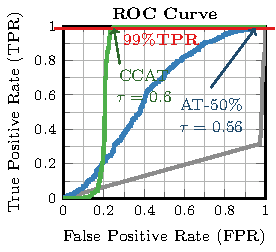
\includegraphics[width=1.05\textwidth]{fig_msvhn_roc}
    \end{minipage}
    \begin{minipage}[t]{0.25\textwidth}
        \vspace*{0px}
        
        \centering			
        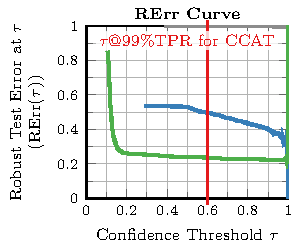
\includegraphics[width=1.05\textwidth]{fig_msvhn_rte}
    \end{minipage}\\
    
    \hspace*{-0.4cm}
    \begin{minipage}[t]{0.45\textwidth}
        \fbox{
            \hspace*{1.6cm}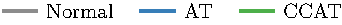
\includegraphics[width=0.575\textwidth]{fig_msvhn_legend}\hspace*{1.6cm}
        }
    \end{minipage}
    \vskip -4px
    \caption{\textbf{ROC and \RTE Curves.} On SVHN, we show ROC curves when distinguishing \emph{correctly classified} test examples from adversarial examples by confidence (left) and (confidence-thresholded) \RTE against confidence threshold $\tau$ (right) for worst-case adversarial examples across $L_\infty$ attacks with $\epsilon = 0.03$. The confidence threshold $\tau$ is chosen exclusively on correctly classified clean examples to obtain $99\%$TPR. For \ConfTrain, this results in $\tau \approx 0.6$. Note that \RTE subsumes both \TE and FPR.}
    \label{fig:experiments-evaluation}
    \vspace*{-2px}
\end{figure}

\textbf{Per-Example Worst-Case Evaluation:}
%
Instead of reporting average or per-attack results, we use a per-example \emph{worst-case} evaluation scheme: For each individual test example, all adversarial examples from all attacks (and restarts) are accumulated. Subsequently, \emph{per test example}, only the adversarial example with highest confidence is considered, resulting in a significantly stronger robustness evaluation compared to related work.